\documentclass[14pt,aspectratio=169,hyperref={pdftex,unicode},xcolor=dvipsnames]{beamer}
\usepackage[english,russian]{babel}
\usepackage[utf8x]{inputenc}
\usepackage[T2A]{fontenc}
\usepackage{cmap}
\usepackage{paratype}
\usepackage{minted} % для примеров кода (требует параметра -shell-escape)
\usepackage{multicol}
\usepackage{qrcode}

\usetheme{metropolis}
\usefonttheme[]{professionalfonts}  % запрещаем beamer'у перезаписывать мат. шрифты
\metroset{numbering=fraction}
\metroset{subsectionpage=progressbar}

\setbeamercolor{frametitle}{fg=black}
\setbeamertemplate{frametitle}
{
 \vspace{3mm}\insertframetitle\par
}
\setbeamertemplate{title separator}{}
\setbeamertemplate{footnote separator}{}


\usebackgroundtemplate{\includegraphics[width=\paperwidth,height=\paperheight]{./common/background_white.jpg}}

\logo{\vspace{-1.2cm}\includegraphics[width=6mm]{./common/short-v.pdf}\hspace*{1.08\textwidth}}

\institute
{
  \begin{columns}
    \begin{column}{1.5cm}
    \includegraphics[height=15mm,keepaspectratio]{./common/math-cs.pdf}
    \end{column}
    \begin{column}{4cm}
          Факультет математики и компьютерных наук СПбГУ
    \end{column}
  \end{columns}
}
\newcommand{\tabitem}{~~\llap{\textbullet}~~}


\begin{document}

\begin{frame}[plain]
  \begin{center}
    \textbf{Иван Климов}

    {\Large\textbf{Применение SAT-подхода в решении water pouring puzzle}}

    %Выпускная квалификационная работа

    %{\small Научный руководитель: А.\,А.\,Выбегалло}

    04.06.2022
  \end{center}


  \begin{columns}
    \begin{column}{1cm}
    \includegraphics[height=15mm,keepaspectratio]{./common/math-cs.pdf}
    \end{column}
    \begin{column}{10cm}
      \small
          Факультет математики и~компьютерных наук СПбГУ\\
          Программа <<Современное программирование>>
    \end{column}
  \end{columns}
\end{frame}



\begin{frame}
\frametitle{Water pouring puzzle}
\begin{center}
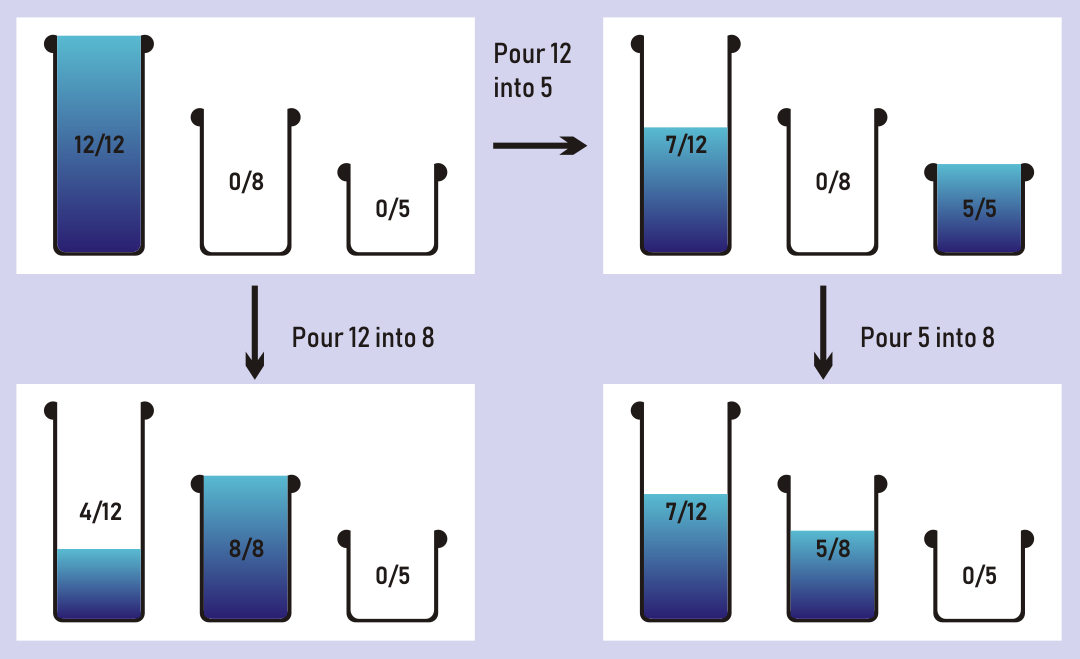
\includegraphics[scale=0.29]{water_pouring_puzzle.png}
\end{center}
\end{frame}

\begin{frame}
\frametitle{Taps and sinks}
\begin{center}
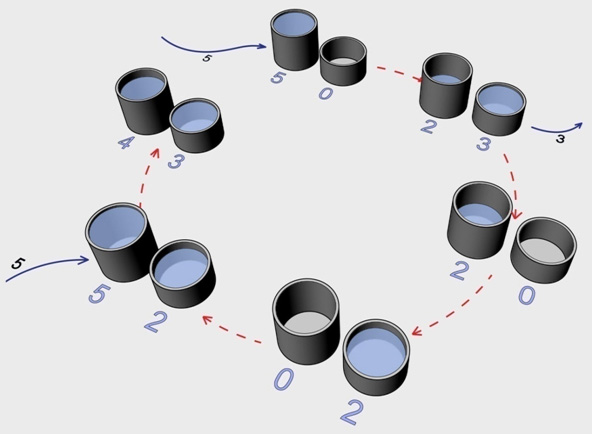
\includegraphics[scale=0.39]{taps_and_sinks.jpg}
\end{center}

\end{frame}

\begin{frame}
\frametitle{Построение формулы для пути длины $k$}
%\begin{itemize}
%  \item $N$ ---  количество кувшинов,
%  \item $v \in \mathbb{Z}^N_{\geq 0}$ --- объемы кувшинов,
%  \item $g \in \mathbb{Z}^N_{\geq 0}$ --- искомое состояние,
%  \item $x_{s, l}$ --- переменная($s \in \mathbb{Z}_{\geq 0}, l \in \mathbb{Z}^N_{\geq 0})$.
%\end{itemize}
  {\small
\begin{tabular}{ll}
  \tabitem $N$ ---  количество кувшинов, & \tabitem $x_{s, l}$ --- переменная($s \in \mathbb{Z}_{\geq 0}, l \in \mathbb{Z}^N_{\geq 0})$, \\
  \tabitem $v \in \mathbb{Z}^N_{\geq 0}$ --- объемы кувшинов, & \tabitem $g \in \mathbb{Z}^N_{\geq 0}$ --- искомое состояние.
\end{tabular}
  }
\vspace{3mm}
\hrule
\vspace{3mm}
Клозы:
\begin{enumerate}
  \item $(x_{0, 0})$,
  \item $(\overline{x_{s, l}} \vee x_{s - 1, l_1} \vee \dotsb \vee x_{s - 1, l_m}),\; \forall s \in \mathbb{Z}_{>0},\forall l \leq v, l_i \rightarrow l$,
  \item $(\overline{x_{s, l}} \vee \overline{x_{s, l'}}),\; \forall s \in \mathbb{Z}_{>0}, \forall l, l' \leq v, l \ne l'$,
  \item $(x_{0, g} \vee x_{1, g} \vee \dotsb \vee x_{k, g})$.
\end{enumerate}
\end{frame}

\begin{frame}
\frametitle{MaxSAT}
\begin{itemize}
  \item WCNF --- CNF с обязательными(hard) и необязательными(soft) клозами:
    \begin{equation*}
      \mathcal{F} = \mathcal{H} \wedge \mathcal{S}
    \end{equation*}
  \item Вес выполняющего набора, который максимизируется:
  \begin{equation*}
    W(x_1, x_2, \dotsc, x_n) = \sum\limits_{c_i \in \mathcal{S}} w_i \cdot c_i(x_1, \dotsc, x_n)
  \end{equation*}
  \item Положим $\mathcal{S} = \bigwedge \overline{x_{s, l}}$.
\end{itemize}
\end{frame}

\begin{frame}
\frametitle{Результаты работы}

\begin{enumerate}
\item Разработан алгоритм сведения Water pouring puzzle к задаче выполнимости.
\item Реализовано консольное приложение с поддержкой различных методов решения задачи.
\end{enumerate}

\vspace{5mm}\hrule\vspace{3mm}

%\begin{center}
%  %Иван Климов, \href{https://github.com/klimoza/taps-and-sinks-solver}{taps-and-sinks-solver} \\
%  \begin{tabular}{c c}
%    Иван Климов & 
\includegraphics[scale=0.19]{qr.png}
%  \end{tabular}
%\end{center}

\begin{multicols}{2}
\begin{center}
  \mbox{}\hfill Иван Климов \href{https://t.me/klimoza}{@klimoza} \\
  \mbox{}\hfill \href{https://github.com/klimoza/taps-and-sinks-solver}{taps-and-sinks-solver}
\end{center}
\columnbreak
\begin{center}
%\qrcode{https://github.com/mtt-lang/mtt-lang}
  %
\includegraphics[scale=0.14]{qr.png}
  \qrcode{https://github.com/klimoza/taps-and-sinks-solver}
\end{center}
\end{multicols}

\end{frame}

\end{document}
